% **************************************************
% Document Class Definition
% **************************************************
\documentclass[%
    paper=A4,               % paper size --> A4 is default in Germany
    twoside=true,           % onesite or twoside printing
    openright,              % doublepage cleaning ends up right side
    parskip=half,           % spacing value / method for paragraphs
    chapterprefix=true,     % prefix for chapter marks
    11pt,                   % font size
    headings=normal,        % size of headings
    bibliography=totoc,     % include bib in toc
    listof=totoc,           % include listof entries in toc
    titlepage=on,           % own page for each title page
    captions=tableabove,    % display table captions above the float env
    chapterprefix=false,    % do not display a prefix for chapters
    appendixprefix=false,    % but display a prefix for appendix chapter
    draft=false,            % value for draft version
]{scrreprt}%


% **************************************************
% Setup YOUR thesis document in this file !
% **************************************************
% !TEX root = main.tex


% **************************************************
% Files' Character Encoding
% **************************************************
\PassOptionsToPackage{utf8}{inputenc}
\usepackage{inputenc}


% **************************************************
% Information and Commands for Reuse
% **************************************************
\newcommand{\thesisTitle}{Esercitazione di laboratorio su progetto di cablaggio strutturato e rete locale}
\newcommand{\thesisName}{Riccardo Persello}
\newcommand{\thesisSubject}{Reti di Calcolatori}
\newcommand{\thesisDate}{\today}
\newcommand{\thesisVersion}{1.0}

\newcommand{\thesisFirstSupervisor}{Pier Luca Montessoro}

\newcommand{\thesisUniversity}{\protect{Università degli Studi di Udine}}
\newcommand{\thesisUniversityDepartment}{Dipartimento di Ingegneria e Architettura}
\newcommand{\thesisUniversityGroup}{Corso di Ingegneria Elettronica}


% **************************************************
% Debug LaTeX Information
% **************************************************
%\listfiles


% **************************************************
% Load and Configure Packages
% **************************************************
\usepackage[italian]{babel} % babel system, adjust the language of the content
\PassOptionsToPackage{% setup clean thesis style
    figuresep=colon,%
    hangfigurecaption=false,%
    hangsection=true,%
    hangsubsection=true,%
    sansserif=false,%
    configurelistings=true,%
    colorize=full,%
    colortheme=bluemagenta,%
    configurebiblatex=true,%
    bibsys=biber,%
    quotesstyle=italian,%
    bibfile=bibliography,%
    bibstyle=numeric,%
    bibsorting=nty,%
}{cleanthesis}
\usepackage{cleanthesis}

\hypersetup{% setup the hyperref-package options
    pdftitle={\thesisTitle},    %   - title (PDF meta)
    pdfsubject={\thesisSubject},%   - subject (PDF meta)
    pdfauthor={\thesisName},    %   - author (PDF meta)
    plainpages=false,           %   -
    colorlinks=false,           %   - colorize links?
    pdfborder={0 0 0},          %   -
    breaklinks=true,            %   - allow line break inside links
    bookmarksnumbered=true,     %
    bookmarksopen=true          %
}

\bibliography{bib-refs}
\renewcommand\lstlistlistingname{Elenco dei listati}

\usepackage{siunitx}
\sisetup{detect-all}


% **************************************************
% Document CONTENT
% **************************************************
\begin{document}

% uncomment the following command to fill up pages with
% whitespace instead of aligning the first and last lines
% of a page (see \raggedbottom vs. \flushbottom)
%\raggedbottom

% --------------------------
% rename document parts
% --------------------------
%\renewcaptionname{ngerman}{\figurename}{Abb.}
%\renewcaptionname{ngerman}{\tablename}{Tab.}
%\renewcaptionname{english}{\figurename}{Fig.}
%\renewcaptionname{english}{\tablename}{Tab.}
\renewcaptionname{italian}{\figurename}{Fig.}
\renewcaptionname{italian}{\tablename}{Tab.}

% --------------------------
% Front matter
% --------------------------
\pagenumbering{roman}			% roman page numbing (invisible for empty page style)
\pagestyle{empty}				% no header or footers
% !TEX root = ../my-thesis.tex
%
% ------------------------------------  --> cover title page
\begin{titlepage}
	\pdfbookmark[0]{Cover}{Cover}
	\flushright\hfill
	\vfill
	{\LARGE\thesisTitle\par}
	\rule[5pt]{\textwidth}{.4pt} \par
	{\Large\thesisName}
	\vfill
	\textit{\large\thesisDate} \\
	% Version: \thesisVersion
\end{titlepage}


% ------------------------------------  --> main title page
\begin{titlepage}
	\pdfbookmark[0]{Titlepage}{Titlepage}
	\tgherosfont\centering

	% {\Large \thesisUniversity} \\[4mm]
	
\includegraphics[width=6cm]{gfx/uniud.jpeg} \\[2mm]
	\textsf{\thesisUniversityDepartment} \\
	\textsf{\thesisUniversityGroup} \\

	\vfill
	{\large \thesisSubject} \\[5mm]
	{\LARGE \color{ctcolortitle}\textbf{\thesisTitle} \\[10mm]}
	{\Large \thesisName} \\

	\vfill

	\normalfont\flushleft{
		\small
		\textbf{\thesisName}\\
		\textit{\thesisTitle}\\
		\thesisSubject, \thesisDate\\
		Docente: \thesisFirstSupervisor\\[1.5em]
		\textbf{\thesisUniversity}\\
		\thesisUniversityDepartment\\
		\thesisUniversityGroup\\
	}
\end{titlepage}
		% INCLUDE: all titlepages
\cleardoublepage{}

\pagestyle{plain}				% display just page numbers
% !TEX root = ../my-thesis.tex
%
\pdfbookmark[0]{Abstract}{Abstract}
\addchap*{Abstract}
\label{sec:abstract}

\blindtext

\vspace*{20mm}

{\usekomafont{chapter}Abstract (different language)}
\label{sec:abstract-diff}

\blindtext
		% INCLUDE: the abstracts (english and german)
\cleardoublepage{}
%
% % !TEX root = ../my-thesis.tex
%
\pdfbookmark[0]{Acknowledgement}{Acknowledgement}
\addchap*{Acknowledgement}
\label{sec:acknowledgement}

\Blindtext[2][2]
 % INCLUDE: acknowledgement
% \cleardoublepage{}
%
\currentpdfbookmark{\contentsname}{toc}
\setcounter{tocdepth}{2}		% define depth of toc
\tableofcontents				% display table of contents
\cleardoublepage{}

% --------------------------
% Body matter
% --------------------------
\pagenumbering{arabic}			% arabic page numbering
\setcounter{page}{1}			% set page counter
\pagestyle{scrheadings}			% header and footer style

%% Uncomment the following lines using the \part command
%% to add part sections
% \part{Example Part}
% % !TEX root = ../../../main.tex
%

\chapter{Cablaggio Strutturato}
Inserire descrizione.   % INCLUDE: 1 - introduction
% % !TEX root = ../../../main.tex
%

\section{Analisi}
Prima di procedere con la prima parte del progetto, è necessario analizzare collettivamente
le planimetrie ed i requisiti indicati. Si sceglie di iniziare dai requisiti necessari a soddisfare
gli utenti finali di questo progetto, ovvero i dipendenti aziendali (ed in genere chiunque debba collegarsi
alla rete in questione). Dal punto di vista del cablaggio strutturato, il vincolo è dato principalmente dalle
postazioni e dalle apparecchiature da collegare alla rete cablata, in quanto richiederanno un numero minimo
ben preciso di prese a muro necessarie a garantire il loro collegamento assieme ad una ridondanza
sufficientemente elevata. Questo si rivela utile al fine di scongiurare interventi eccessivamente lunghi,
costosi ed invasivi nell'eventualità del danneggiamento di una linea od un apparato di rete.

\subsection{Conteggio delle prese utente}   % INCLUDE: 1 - analysis
% !TEX root = ../../../main.tex
%

\newpage
\section{Progettazione}
\subsection{Tipo di presa}

\begin{wrapfigure}{r}{5cm}
  \centering
  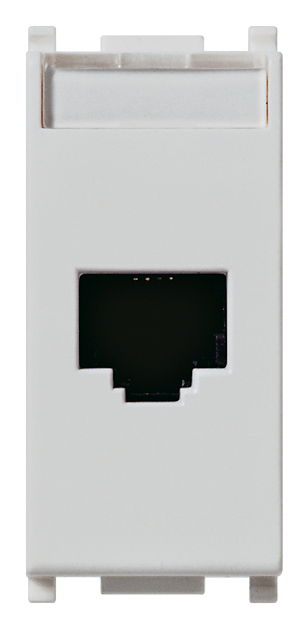
\includegraphics{vimar-14338-8-SL.jpg}
  \caption{Il connettore scelto per le prese utente.}\label{fig:presa}
\end{wrapfigure}

Supponendo che l'edificio abbia già alcune scatole elettriche incassate dedicate all'impianto di rete,
dove necessarie (anche condivise con altri connettori/controlli), non si terrà conto del costo di queste ultime.

Si sceglie di utilizzare prodotti di marca Vimar, serie Netsafe.
Nello specifico, si sceglie di usare dei connettori RJ45 Cat5e UTP (codice 14338.8.SL), illustrato in figura~\ref{fig:presa}.

Dato che determinate scatole elettriche possono contenere anche prese, pulsanti, interruttori o altri tipi
di dispositivi, non si conosce la dimensione (e di conseguenza il costo) delle placche decorative e dei supporti di montaggio.

Si suppone pertanto di affidarsi a quanto già predisposto per l'impianto elettrico (ove possibile).

Notare che nella maggior parte dei casi, questo non sarà necessario, in quanto gran parte dell'impianto,
per motivi di flessibilità e semplicità, verrà posato a pavimento, con delle prese direttamente disponibili sulle scrivanie.

Nei casi in cui è invece necessario affidarsi a delle prese a muro, resta valido quanto prima descritto.

\subsection{Dislocazione degli armadi e dorsale principale}

Data la topografia stellare del cablaggio orizzontale, si preferisce ospitare gli armadi per la \textit{floor distribution}
nei locali tecnici centrali all'edificio, in ogni piano. Essendo già stato fissato dalla planimetria fornita, il centralino
telefonico sarà per forza posizionato nel locale tecnico sud-ovest del piano terreno, assieme alle apparecchiature per
il collegamento alla rete pubblica.

Con questa scelta, il server (posizionato al piano terreno), godrà di una distanza ridotta con l'armadio di piano, garantendo
un miglior collegamento (in quanto si assume che il server necessiti di una considerevole quantità di banda), ed una maggiore
flessibilità nel caso in cui, in futuro, dovessero essere necessarie delle espansioni.

I collegamenti di dorsale dell'edificio saranno inizialmente orizzontali, dirette dal locale tecnico sud-ovest del piano terreno
verso quello centrale. Da quel punto, si muoveranno in verticale, raggiungendo gli altri armadi. La stessa cosa vale per i collegamenti
addizionali tra armadi adiacenti.

\subsection{Cablaggio orizzontale}

Si suppone di avere a disposizione un sistema di cablaggio a pavimento galleggiante, comprensivo di più canalette di larghezza sufficientemente
ampia da poter accogliere complessivamente, nelle parti iniziali del percorso, circa la metà di tutti i cavi utilizzati nel cablaggio di un singolo piano.

Per quanto concerne la sala riunioni, essendo adiacente al locale tecnico contenente l'armadio, ed essendo dotata di numerose prese,
si preferisce evitare di dover passare il cablaggio attraverso il corridoio: si preferisce attraversare il muro, predisposto con
un foro di diametro sufficiente, per raggiungere i tavoli da sotto il pavimento. Qui, le connessioni saranno poste al centro del tavolo principale
e su quello del presentatore mediante delle scatole elettriche oblique da scrivania.

Si ritiene utile sfruttare un passaggio simile per il raggiungimento della vicina sala server e, per i piani superiori,
del corridoio al lato opposto della porta presente nel locale tecnico. Non si ritiene ragionevole il percorrimento a ``U'' del corridoio
principale per il solo fine di raggiungere degli uffici altrimenti molto vicini in linea d'aria.

Queste considerazioni sono riportate nelle planimetrie che seguono (figure~\ref{fig:planimetria-terreno-cablaggio}~e~\ref{fig:planimetria-1-cablaggio}). I cablaggi di dorsale sono tracciati con delle linee
di spessore maggiore, ed i cerchi indicano il passaggio tra piani differenti.

Gli armadi sono evidenziati in azzurro e le prese in fuchsia.

Il cablaggio si distingue nel seguente modo:
\begin{description}
  \item[Verde] Fibra ottica multimodale 50/125.
  \item[Arancione] Cavi in rame Cat5e per Ethernet.
  \item[Rosso] Cavi in rame voice-grade (Cat3) per fonia.
\end{description}

\begin{figure}[ht]
  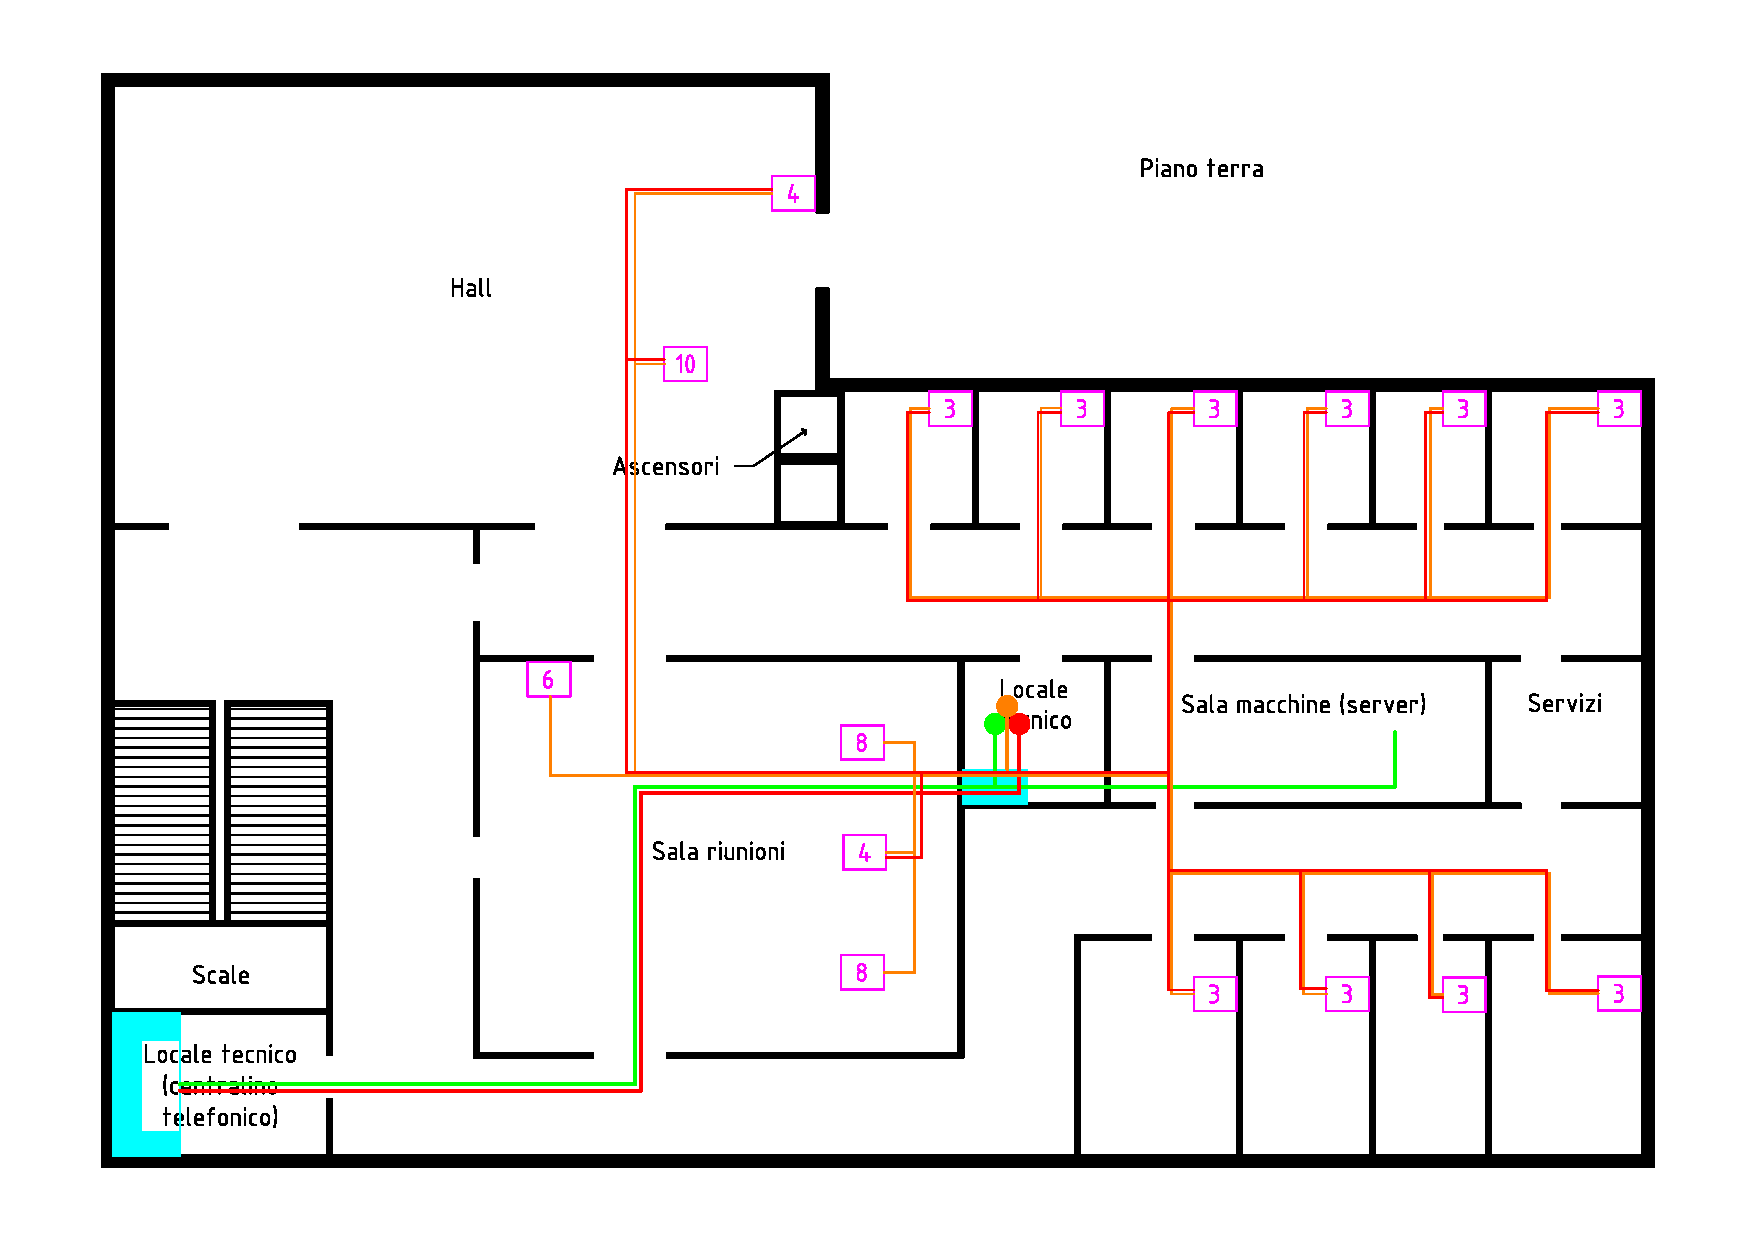
\includegraphics[angle=90,origin=c,width=\textwidth]{planimetrie-pianoterra-cablaggio}
  \caption{Cablaggio del piano terreno.}\label{fig:planimetria-terreno-cablaggio}
\end{figure}

\begin{figure}[ht]
  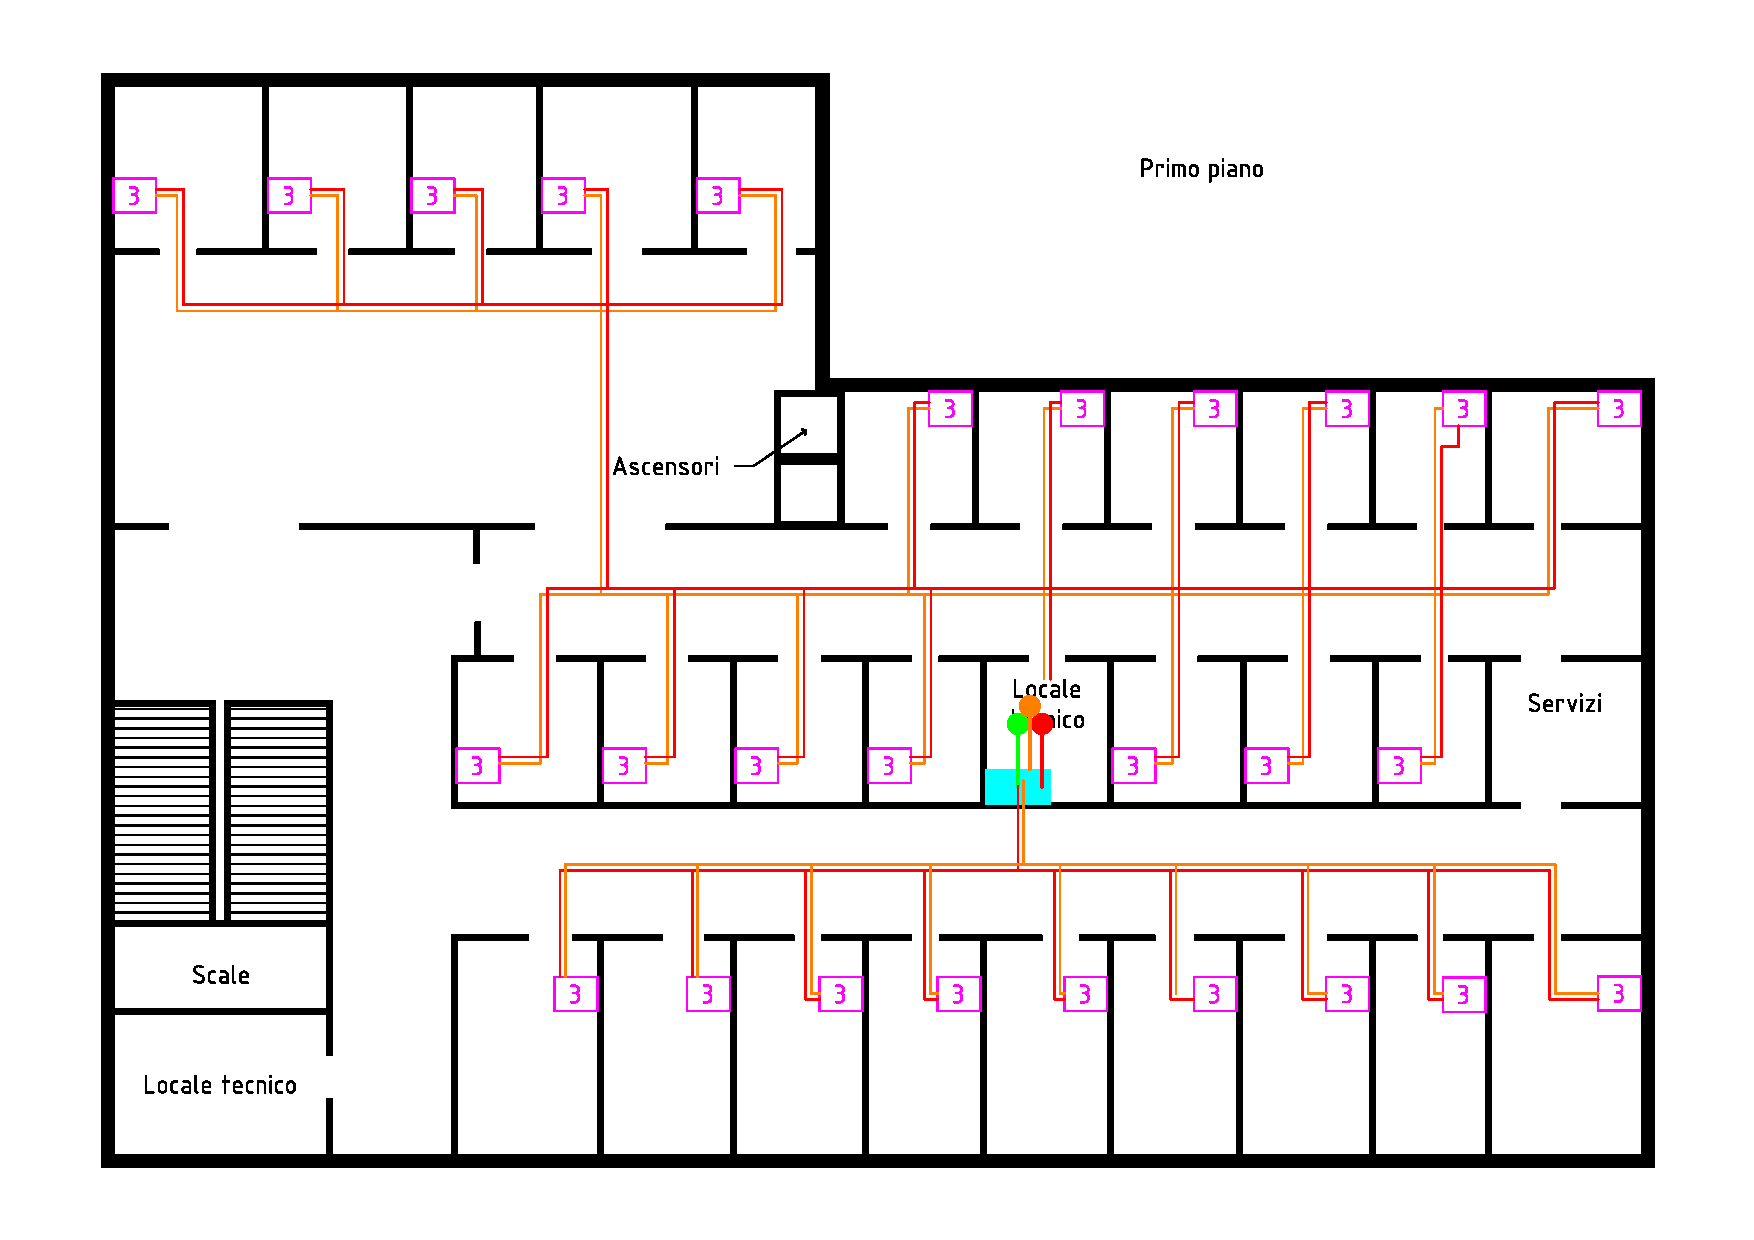
\includegraphics[angle=90,origin=c,width=\textwidth]{planimetrie-piano1-cablaggio}
  \caption{Cablaggio dei piani da primo a quarto.}\label{fig:planimetria-1-cablaggio}
\end{figure}

Si contano due pareti attraversate nel piano terra, e soltanto una per piano nei superiori.
   % INCLUDE: 1 - project

% --------------------------
% Back matter
% --------------------------
%
{%
    \setstretch{1.1}
    \renewcommand{\bibfont}{\normalfont\small}
    \setlength{\biblabelsep}{0pt}
    \setlength{\bibitemsep}{0.5\baselineskip plus 0.5\baselineskip}
    \printbibliography[nottype=online]
    \newrefcontext[labelprefix={@}]
    \printbibliography[heading=subbibliography,title={Webpages},type=online]
}

\cleardoublepage{}

\listoffigures
\cleardoublepage{}

\listoftables
\cleardoublepage{}

\lstlistoflistings{}
\cleardoublepage{}

% \appendix\cleardoublepage{}
% \input{content/chapters/appendix}       % INCLUDE: appendix

\cleardoublepage{}
% !TEX root = ../my-thesis.tex
%
\pagestyle{empty}
\hfill
\vfill
\pdfbookmark[0]{Colophon}{Colophon}
\section*{Colophon}

This thesis was typeset with \LaTeXe.
It uses the \textit{Clean Thesis} style developed by Ricardo Langner.
The design of the \textit{Clean Thesis} style is inspired by user guide documents from Apple Inc.

Download the \textit{Clean Thesis} style at \url{http://cleanthesis.der-ric.de/}.


% \cleardoublepage{}
% % !TEX root = ../my-thesis.tex
%
%************************************************
% Declaration
%************************************************
\pdfbookmark[0]{Declaration}{Declaration}
\addchap{Declaration}
\label{sec:declaration}
\thispagestyle{empty}

You can put your declaration here, to declare that you have completed your work solely and only with the help of the references you mentioned.

\bigskip

\noindent\textit{\thesisUniversityCity, \thesisDate}

\smallskip

\begin{flushright}
	\begin{minipage}{5cm}
		\rule{\textwidth}{1pt}
		\centering\thesisName
	\end{minipage}
\end{flushright}

%*****************************************
%*****************************************

% \clearpage

% \newpage
% \mbox{}

% **************************************************
% End of Document CONTENT
% **************************************************
\end{document}
